%\documentclass{article}
\documentclass[11pt]{scrartcl}
\usepackage[utf8]{inputenc}

% Packages
\usepackage[backend=biber,style=authoryear-icomp,sorting=ynt]{biblatex}
\usepackage{hyperref}
\usepackage{graphicx}
%\usepackage[margin=1.25in]{geometry}
\usepackage{palatino}

% Python Source Code
\usepackage{tcolorbox}
\tcbuselibrary{minted,breakable,xparse,skins}

\definecolor{bg}{gray}{0.95}
\DeclareTCBListing{mintedbox}{O{}m!O{}}{%
  breakable=true,
  listing engine=minted,
  listing only,
  minted language=#2,
  minted style=default,
  minted options={%
    linenos,
    gobble=0,
    breaklines=true,
    breakafter=,,
    fontsize=\small,
    numbersep=8pt,
    #1},
  boxsep=0pt,
  left skip=0pt,
  right skip=0pt,
  left=25pt,
  right=0pt,
  top=3pt,
  bottom=3pt,
  arc=5pt,
  leftrule=0pt,
  rightrule=0pt,
  bottomrule=2pt,
  toprule=2pt,
  colback=bg,
  colframe=orange!70,
  enhanced,
  overlay={%
    \begin{tcbclipinterior}
    \fill[orange!20!white] (frame.south west) rectangle ([xshift=20pt]frame.north west);
    \end{tcbclipinterior}},
  #3}

% Parameters
\hypersetup{
	citecolor={blue},
	linkcolor={red},
}

% Bib Settings
\addbibresource{literature.bib}

\title{Investigating the Impact of Syntactic Features for Semantic Dependency Parsing}
\author{Maximilian Pfundstein}
\date{\today}

\begin{document}

\maketitle
\begin{abstract}

The theoretical baseline model provided by Dozat and Manning (\cite{zeman-etal-2017-conll}) and the implementation from Daniel Roxbo (\cite{Roxbo1315439}) are used for predicting syntactic and semantic dependency graphs. For both, one BiLSTM is being trained and their performance is evaluated in a multitask learning setup. The original model, semantic only, results in an $F_1$ score of $87.50\%$ for an out-of-domain test data set. The multitask model using raw edge matrices achieves an $F_1$ score of $87.80\%$ and another approach using a feedback loop, providing previous learnt semantic as an input for the syntactic scorer, results in an $F_1$ score of $87.87\%$. Thus, multitask learning improves the results, but not significantly. Additionally, the implementation from Daniel Roxbo (\cite{Roxbo1315439}) has been updated to provide faster startup times and the ability to read \texttt{.conllu} files. An existing library called \textit{CoNLL-U Parser} is being used for this functionality and some features have been provided for the library via pull-requests on GitHub.

\end{abstract}

\clearpage

\tableofcontents

\clearpage

\vspace*{\fill}

\textbf{Scope}

The purpose of this report is to summarise the obtained results during the research project (732A76) which is a course of the masters programme in \textit{Statistics and Machine Learning} at Linköpings University in 2019. It therefore assumes that the reader is familiar with the named references, the code base and terms associated with it.

\vspace*{\fill}

\clearpage

\section{Introduction}

Syntactic and semantic dependency parsing (SDP) within the domain of NLP (Natural Language Processing) is the task of creating a directed acyclic graph consisting of nodes and edges to embed the grammatical meaning of a sentence. The research question being investigated here is, if for the prediction of semantic dependencies syntactic information can be utilised and to which extend they provide information for increasing the accuracy of a model.

For answering that question and conducting research, the baseline model originally provided by Dozat and Manning (\cite{zeman-etal-2017-conll}) is being used. The replicated implementation from Daniel Roxbo (\cite{Roxbo1315439}) has been extended during his thesis to be able to also learn syntactic graphs which are provided as features for the semantic dependency parser. The results show that while syntactic gold graphs increase the performance of the semantic parser from 93.6 percent to 97.1 percent, predicted syntactic trees yield in a slightly lower $F_1$ score of 92.8 percent (\cite[p. 33]{Roxbo1315439}). These scores relate to in-domain data.

Further research by \cite{kurtz-etal-2019-improving} suggests that there is an overlap between syntactic and semantic information. This would explain the results provided by (\cite[p. 33]{Roxbo1315439}) and indicate that no further information can be extracted. Other research suggests, that multitask learning can actually improve the results of a solely semantic parser (\cite{peng-etal-2017-deep}). There, the same theoretical model is being used which was applied by Dozat and Manning (\cite{zeman-etal-2017-conll}) and the data utilised is the same as used by \cite{Roxbo1315439}. Then, multitask learning is being applied and higher $F_1$ scores, compared to a solely semantic parser, are achieved.

It should be noticed that the results from \cite{peng-etal-2017-deep} are lower for the multitask learning compared to the pure semantic parser implemented by Robin Roxbo (\cite{Roxbo1315439}). This might be due to a smaller model or a difference in implementation. This research project will not dive deeper into the differences of the implementations, but will focus on examining a multitask learning approach using the implementation from Robin Roxbo (\cite{Roxbo1315439}) to investigate, if the semantic parser can be further improved using predicted syntax.

To further elaborate on this, multitask learning will be utilised to learn the syntactic and semantic scores at the same time while using an interpolated loss. Additionally, another extension to this approach will be tested, which will feed the semantic output back to the syntactic scorer.

\section{Overview}

This research project\footnote{https://www.ida.liu.se/~732A76/index.en.shtml} is embedded in a course of the Masters Programme in Statistics and Machine Learning at Linköpings University\footnote{https://liu.se/en/education/program/f7msl} in 2019 and represents a course\footnote{https://www.ida.liu.se/\~732A76/info/courseinfo.en.shtml}. Therefore, this report also contains improvements to the existing code base which will also be presented in the following chapters. This mainly includes improvements to the existing code base.

The official objectives for this research project have been formalised in the following way:

\begin{quote}
The goal of the project is to investigate the impact of syntactic features for semantic dependency parsing. While it is already known that syntactic features help, previous experiments have shown that predicting syntactic structure, and to then use it as a feature for semantic parsing does not increase performance.

The role of the student is to modernize an existing system, adjust it to read combined syntax-semantic input data, and investigate how to successfully add syntactic features to semantic dependency parsing. This involves testing different neural network variations, pipeline processing and multitask learning.
\end{quote}

During the project the following three objectives have been formulated:

\begin{itemize}
    \item Allow to import the data from the \texttt{.conllu} format.
    \item Increase the performance during the pre-processing by using caching to save computation time.
    \item Implement multitask learning to simultaneously learn syntactic and semantic graphs and investigate the results.
\end{itemize}

The following chapter will explain the different tasks further and which work has been done in detail. The subsequent chapter will present the results of the three objectives and the final chapter includes discussions, conclusions and suggestions.

\section{Objectives}

This chapter will introduce which work has be done for all of the objectives of this research project.

\subsection{.conllu Format}

The implementation from Robin Roxbo (\cite{Roxbo1315439}) reads the syntactic graphs from \texttt{.cpn} and the semantic graphs respectively from \texttt{.sdp} files. Both formats can be seen in figure \ref{fig:syntax_format} and figure \ref{fig:semantic_format}. The aim is to support the CoNLL-U format\footnote{https://universaldependencies.org/format.html} which is based on \cite{10.5555/1596276.1596305}. The format embeds both syntactic and semantic graphs and related information. Furthermore, the support for \texttt{.cpn} and \texttt{.sdp} is being discontinued.

\begin{figure}[hbt]
	\center
	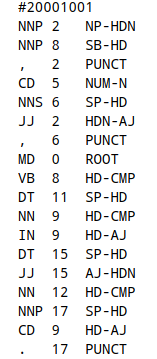
\includegraphics[width=0.2\textwidth]{img/syntax_format}
	\caption{\texttt{.cpn} format (syntax)}
	\label{fig:syntax_format}
\end{figure}

\begin{figure}[hbt]
	\center
	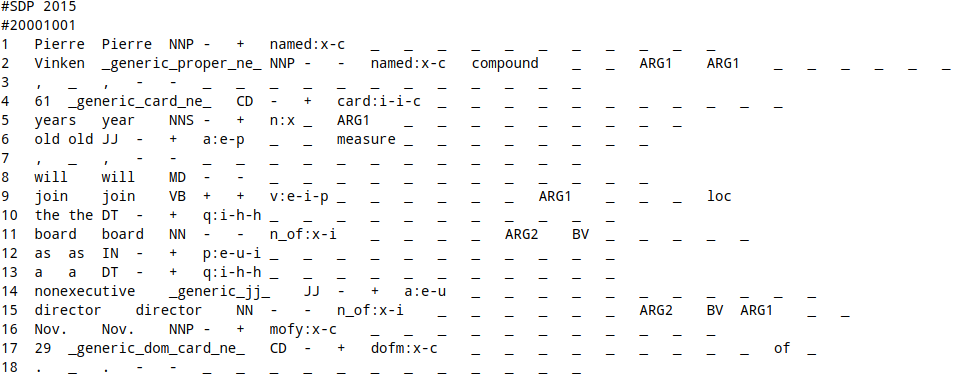
\includegraphics[width=1.0\textwidth]{img/semantic_format}
	\caption{\texttt{.sdp} format (semantic)}
	\label{fig:semantic_format}
\end{figure}

The data is provided in \texttt{.conllu} format along with a sparse implementation for parsing. To fully support \texttt{.conllu} it has to be decided if the already present code is being further utilised, rewritten or if other implementations exist. The library \textit{CoNLL-U Parser}\footnote{https://github.com/EmilStenstrom/conllu} is freely available on GitHub, supports all necessary features and has a good test coverage. Therefore it has been decided to adopt the library and use it for the existing code base.

\begin{figure}[hbt]
	\center
	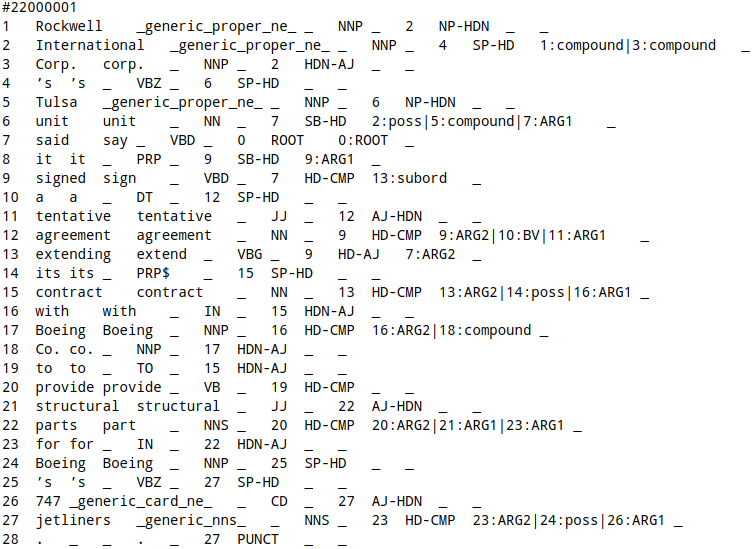
\includegraphics[width=1.0\textwidth]{img/conllu_format}
	\caption{\texttt{.conllu} format (semantic and syntactic)}
	\label{fig:conllu_format}
\end{figure}

During the implementation two problems have been encountered. First, the labels for the edges contain uppercase letters and numbers (compare figure \ref{fig:conllu_format}) which are not officially supported by the CoNLL-U specification. After discussion with the maintainer of the library it was decided to add support for uppercase letters and numbers as there was, apart from not strictly following the specification, no argument against it. The changes\footnote{Issue: https://github.com/EmilStenstrom/conllu/issues/34} have been submitted via pull-request\footnote{Pull Request: https://github.com/EmilStenstrom/conllu/commit/532624b1b897d6167e0da99b4944c345ae04609c} on GitHub.

Secondly, the sentence Ids, which precede each sentence in all formats, are also contrary to the specification. The Ids can be seen in figure \ref{fig:syntax_format}, figure \ref{fig:semantic_format} and figure \ref{fig:conllu_format} in the first row respectively. After evaluation with the library maintainer, a custom fallback parser has been added by the maintainer to handle arbitrary formats of meta information\footnote{https://github.com/EmilStenstrom/conllu\#customizing-parsing-to-handle-strange-variations-of-conll-u}. Furthermore, the row containing the ill-formatted sentence Id has been refactored to be in accordance with the specification. Thus, the row containing the valid sentence Id has the following format after the change: \texttt{\# sent-id = 20001001}. A small Python script has been written to reformat the existing \texttt{.conllu} files. It can be found in appendix \ref{sec:python_script_sentence_ids}.

\subsection{Performance Increase}

Every time the source code is being invoked, the pre-processing is performed again which causes a delay of a few minutes before the task can be executed. Here a task can be for example training or predicting. As the steps for the pre-processing are the same every time, the results are supposed to be cached.

An investigation of the source code led to three functions which are being modified to support caching. These are \texttt{parse\_conllu\_labels}, \texttt{parse\_conllu\_sentences} and \texttt{parse\_conllu\_targets}. Pythons \texttt{pickle} \footnote{https://docs.python.org/3/library/pickle.html} module is being used to cache the results to disk, where the binary format is then being loaded when the method is being invoked again. Some methods are being invoked multiple times, for example when called for the training and development data sets. In addition, an option has been added to disable caching if desired.

\subsection{Multitask Learning}

\begin{figure}[hbt]
	\center
	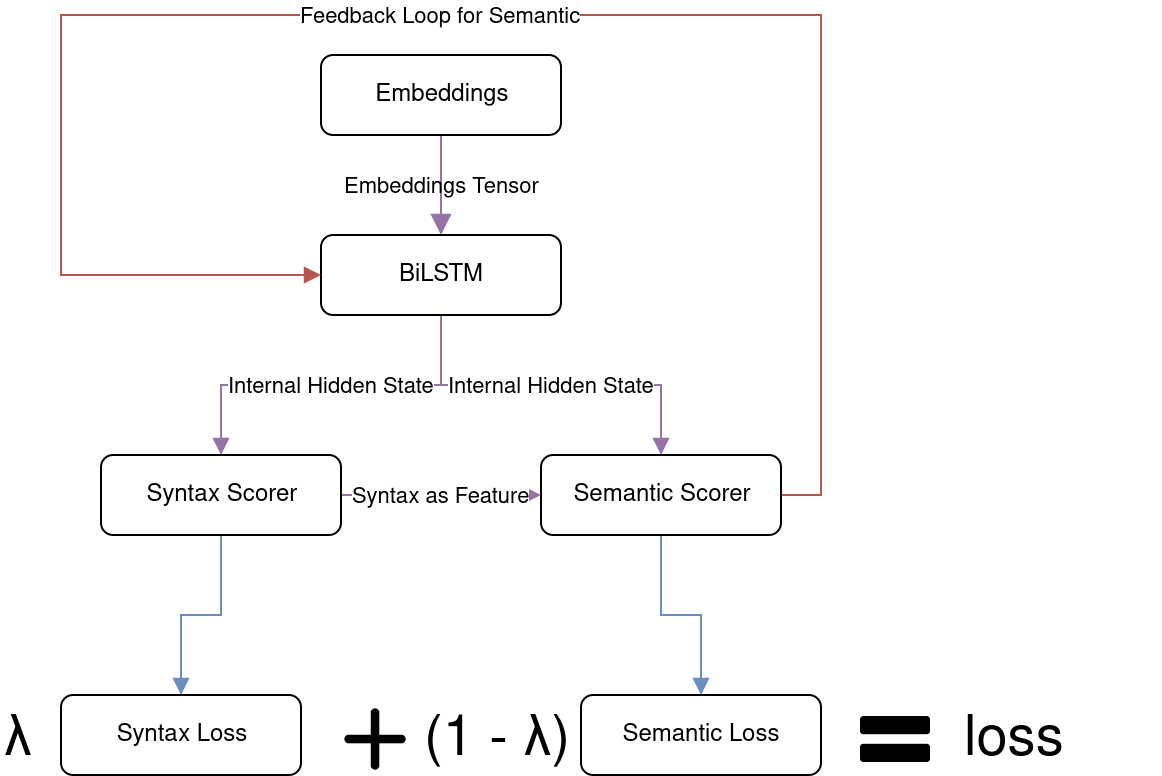
\includegraphics[width=1.0\textwidth]{img/flowchart}
	\caption{Flowchart, with red representing the feedback loop.}
	\label{fig:flowchart}
\end{figure}

As suggested in \cite{kurtz-etal-2019-improving}, multitask learning is implemented for evaluating if predicted syntax can improve the semantic score in this setting. Two approaches have been implemented and will be presented in this chapter. As the model is likely to capture more information, the hyperparameters have been adjusted to account for that. In particular, the 3 layers of the LSTM (Long Short-Term Memory) have been increased extended to 4 layers and the \texttt{hidden\_lstm} and \texttt{hidden\_char\_lstm} have been increased from 400 to 600. The full list of hyperparameters can be found in appendix \ref{sec:hyperparameters}.

\subsubsection{Interpolated Score}

The same model is being used twice, once for predicting syntax and once for predicting semantic. First, the model for predicting syntax is being called and the resulting predictions are then utilised as input features for the semantic predictions. The process structure can be seen in figure \ref{fig:flowchart}. Then, a loss is being calculated for each model and the resulting loss is an interpolation between both, which can then be set as a hyperparameter. Both the syntactic and semantic scorer use the same internal representation of information which is the output of the BiLSTM .

Three different variations have been tested. \textit{Multitask Raw} passes the raw syntax edge scores forward, which are positive and negative floating point numbers. \textit{Multitask Single} sets only for each row of the score matrix (thus for each word) the highest edge score to $1.0$, whereas \textit{Multitask Multi} sets all edges to $1.0$ which are greater than $1.0$. The idea behind this approach is that the semantic scorer potentially will benefit from a simpler input representation.

\subsubsection{Feedback Loop}

Building on top of the same concept as the interpolated score, the feedback loop approach performs one forward pass first, for each batch, and then feeds the semantic predictions as features to the syntactic input. This way the syntax scorer might be able to use learned semantic information from previous pass-throughs for further improvement. The structure can be seen in figure \ref{fig:flowchart}, where the red line represents the feedback loop for the semantic information passed back to the BiLSTM so that the syntactic scorer can use it. 

The feedback loop was only tested for \textit{Multitask Raw} as time was limited and \textit{Multitask Raw} looked most promising during testing.

\section{Results}

The results of the three objectives will be presented in this chapter.

\subsection{\texttt{.conllu} Format}

All discussed changes to the library have been adopted by the maintainer of the library. The code base has been modified at several locations, especially as many functions had dependencies on the previous existing tooling functions for reading in the input. Some of the dependencies have been resolved and the code base can now fully rely on the existing library for reading \texttt{.conllu} files.

\subsection{Performance Improvement}

The startup time for the code base could be improved by several seconds. Depending on the task to perform, sometimes even by minutes. Figure \ref{fig:cache_speedup} shows the speedup achieved after implementation of caching for the three main functions of the code base.

The function \texttt{parse\_conllu\_labels} benefited most from the caching, reducing the computational time to $341\mu$s. For the other functions the speedup was not as significant, but still saves several seconds each run. \texttt{parse\_conllu\_sentences} is around $7.93$ times faster and the function \texttt{parse\_conllu\_targets} is around $9.42$ times faster than before.

\begin{figure}[hbt]
	\center
	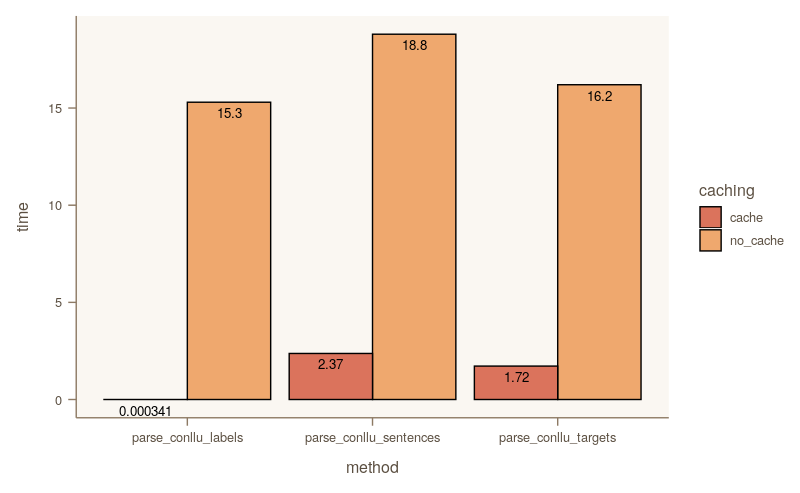
\includegraphics[width=1.0\textwidth]{img/cache_speedup.png}
	\caption{Speedup using caching (time in seconds).}
	\label{fig:cache_speedup}
\end{figure}

\subsection{Multitask Learning}

\begin{figure}[hbt]
	\center
	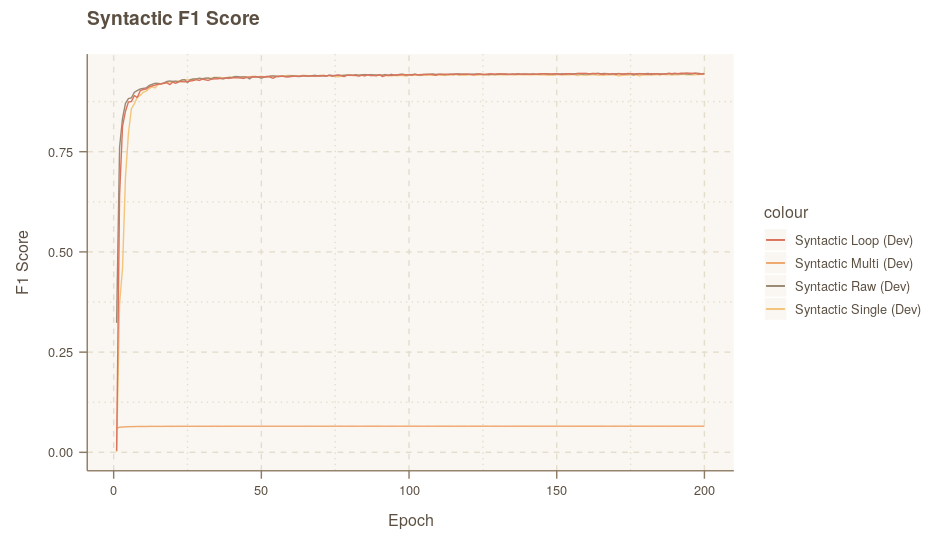
\includegraphics[width=1.0\textwidth]{img/syntactic_f1_200.png}
	\caption{Syntactic $F_1$ score for 200 epochs.}
	\label{fig:syntactic_f1_200}
\end{figure}

\begin{figure}[hbt]
	\center
	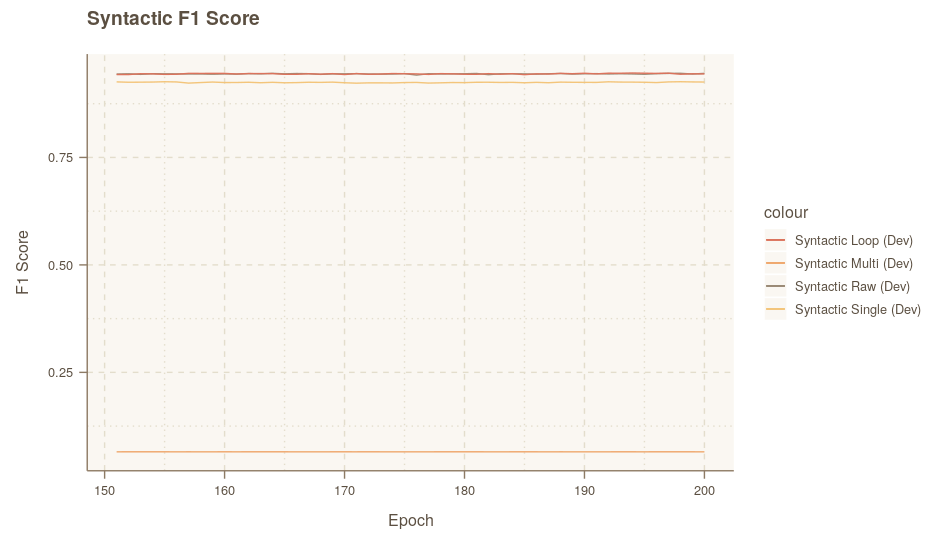
\includegraphics[width=1.0\textwidth]{img/syntactic_f1_50.png}
	\caption{Syntactic $F_1$ score for the last 50 epochs.}
	\label{fig:syntactic_f1_50}
\end{figure}

\begin{figure}[hbt]
	\center
	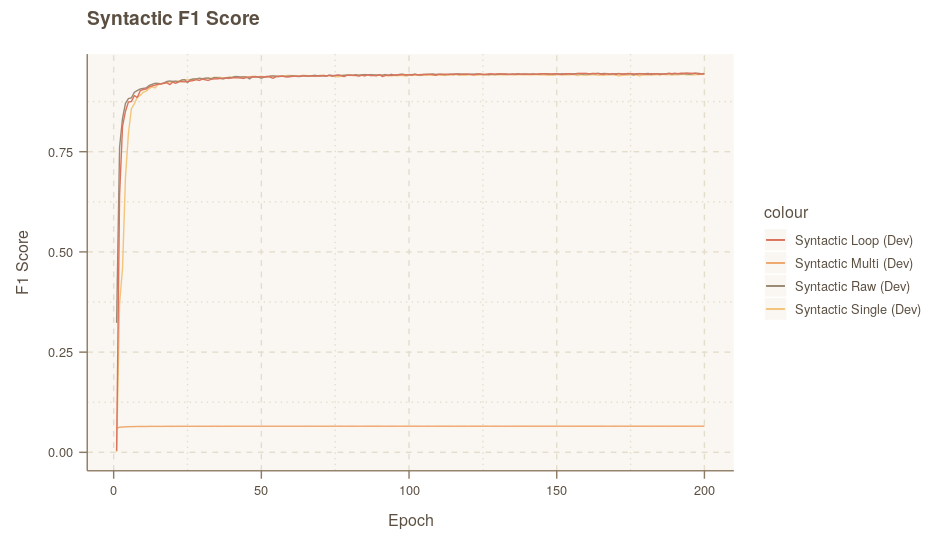
\includegraphics[width=1.0\textwidth]{img/semantic_f1_200.png}
	\caption{Semantic $F_1$ score for 200 epochs.}
	\label{fig:semantic_f1_200}
\end{figure}

\begin{figure}[hbt]
	\center
	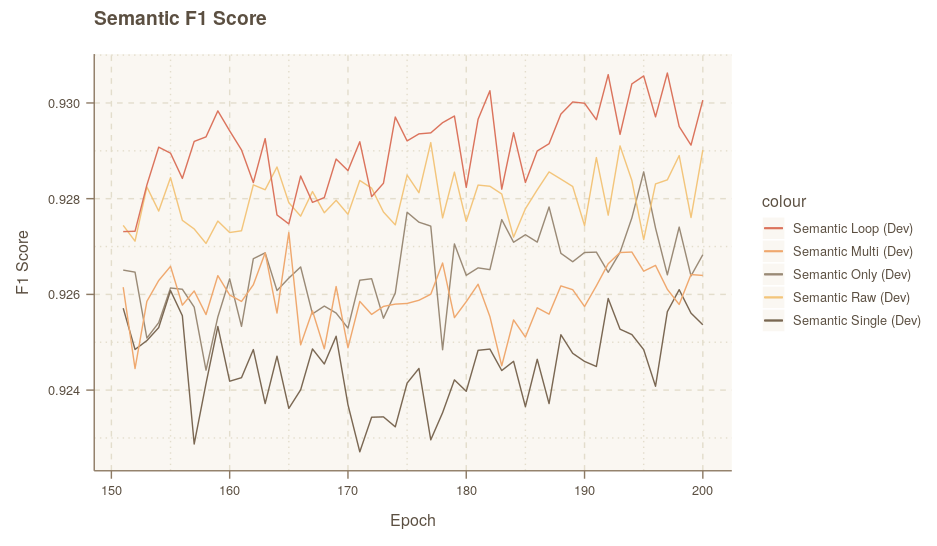
\includegraphics[width=1.0\textwidth]{img/semantic_f1_50.png}
	\caption{Semantic $F_1$ score for the last 50 epochs.}
	\label{fig:semantic_f1_50}
\end{figure}

The $F_1$ scores on the development data set during training can be seen in figure \ref{fig:syntactic_f1_200} for the syntactic $F_1$ scores and in figure \ref{fig:semantic_f1_200} for the semantic $F_1$ scores over 200 epochs. Figure \ref{fig:syntactic_f1_50} and \ref{fig:semantic_f1_50} show the curves for the last 50 epochs.

It can be seen that for the syntactic score, using multiple edges set to $1.0$ (Syntactic Multi), the networks completely fails to learn. For setting just one edge to $1.0$, the network is learning, but it can be seen that it learns slower and reaches a lower $F_1$ score in the end compared to both implementations using raw edge matrices. We therefore conclude that reducing any information about scores yields in lower $F_1$ scores and the assumption, that the semantic scorer benefits from a simpler representation, is wrong.

All semantic versions of the network manage to learn to some good extend. The single semantic version learns slowest while also performing worst. These observations are consistent with the results for the syntactic scorer.

Looking at the last 50 epochs for the semantic scores, it can actually be seen that the different scorers stagnate at different values. A conducted one way ANOVA test also shows with very high significance ($p < 10^{-6}$), that all scorers do not share a common mean for the $F_1$ score. As for the syntactic scorers, the raw edge matrices perform best. Interestingly, the feedback loop seems have a slightly higher $F_1$ score compared to the raw multitask version. Nevertheless, the improvement is very marginal.

\begin{table}[h]
    \centering
    \begin{tabular}{l|r|r|r|r}
        Setting & \textbf{Syn Dev} & \textbf{Sem Dev} & \textbf{Syn Test} & \textbf{Sem Test} \\ \hline
        Sem Only & o & 92.39\% & o & \textbf{87.50\%} \\ 
        Multitask Raw & - & - & 90.92\% & \textbf{87.80\%} \\
        Multitask Single & 94.64\% & 92.6\% & 90.81\% & 87.41\% \\
        Multitask Multi & - & - & 7.39\% & 87.71\% \\
        Multitask Loop & 94.29\% & 92.51\% & 90.96\% & \textbf{87.87\%} \\
    \end{tabular}
    \caption{$F_1$ scores for the different setups.}
    \label{tab:results}
\end{table}

Table \ref{tab:results} shows the final $F_1$ scores for syntax and semantic models for the development and test data set from the best models during the training process. Missing values are denoted with a \textit{minus} and undefined values are defined by the letter \textit{o}. The missing values are available on request, as all models have been saved, but the values have not been logged during evaluation.

It can be seen that multitask learning seems to slightly increase the semantic test score. The \textit{Semantic Only} model achieves an $F_1$ score of $87.50\%$ whereas the multitask learning model using raw edges achieves an $F_1$ score of $87.80\%$ and the feedback loop model achieves a very slightly higher $F_1$ score of $87.87\%$.

\section{Conclusions}

It seems that multitask learning does increase the performance, but not as much as proposed by \cite{peng-etal-2017-deep}. At least in terms of this data set. One of the reasons for this behaviour could be that the model used by \cite{peng-etal-2017-deep} underfits the data, as the presented semantic only scorer (\textit{Semantic Only}) already outperforms the proposed multitask model from \cite{peng-etal-2017-deep}. It could be that the information captured using a multitask approach can also be learned by a model not utilising multitask learning.

The findings of this research project emphasise the presumption of \cite{kurtz-etal-2019-improving} that the syntactic and semantic representation of a sentence indeed share some information.

To further investigate this presumption, one could take a look at Bidirectional Encoder Representations from Transformers (BERT) and see if this pre-trained model achieves higher scores compared to using Global Vectors for Word Representation (GloVe) embeddings. If computational resources are available, BERT could be trained on this specific domain of problem. Another approach could be to combine BERT with multitask learning.

\clearpage

\printbibliography

\clearpage

\section{Appendix}

\subsection{Python Script for Reformatting Sentence Id Rows}
\label{sec:python_script_sentence_ids}

\begin{mintedbox}{python}
import sys
import os

read_path = sys.argv[1]
write_path = sys.argv[1] + ".temp"
with open(read_path, "r", encoding="utf-8") as read_file:
    with open(write_path, "w", encoding="utf-8") as write_file:
        for line in read_file:
            if line[0] == "#" and line[1] != " ":
                line = line[0] + " sent-id = " + line[1:]
            write_file.write(line)

os.rename(write_path, read_path)

\end{mintedbox}

\subsection{Hyperparameters}
\label{sec:hyperparameters}

\subsubsection{Semantic Only}

\begin{mintedbox}{python}

[data]
train                  = data/sdp/en.train.dm.dt.deepbank.conllup
val                    = data/sdp/en.dev.dm.dt.deepbank.conllup
predict_file           = data/sdp/en.id.dm.dt.deepbank.conllup
glove                  = data/glove.6B.100d.txt
#load                   = 
syn_input_style        = none

[training]
batch_size             = 50
epochs                 = 200
beta1                  = 0
beta2                  = 0.95
l2                     = 3e-09

[network_sizes]
hidden_lstm            = 600
hidden_char_lstm       = 600
layers_lstm            = 4
dim_mlp                = 600
dim_embedding          = 100
dim_char_embedding     = 100
early_stopping         = 0

[network]
pos_style              = xpos
target_style           = sem 
attention              = bilinear
synsem_interpolation   = 0.0
loss_interpolation     = 0.025
lstm_implementation    = drop_connect
char_implementation    = convolved
disable_gradient_clip  = False
unfactorized           = True
emb_dropout_type       = replace
score_encoding         = raw

[features]
disable_glove          = False
disable_char           = False
disable_lemma          = True
disable_pos            = False
disable_form           = False

[dropout]
dropout_embedding      = 0.2
dropout_edge           = 0.25
dropout_label          = 0.33
dropout_main_recurrent = 0.25
dropout_recurrent_char = 0.33
dropout_main_ff        = 0.45
dropout_char_ff        = 0.33
dropout_char_linear    = 0.33

[other]
seed                   = 1234
force_cpu              = False

[output]
quiet                  = False
save_every             = False
disable_val_eval       = False
enable_train_eval      = False


\end{mintedbox}

\subsubsection{Multitask Single}

\begin{mintedbox}{python}

[data]
train                  = data/sdp/en.train.dm.dt.deepbank.conllup
val                    = data/sdp/en.dev.dm.dt.deepbank.conllup
predict_file           = data/sdp/en.id.dm.dt.deepbank.conllup
glove                  = data/glove.6B.100d.txt
#load                   = 
syn_input_style        = gold

[training]
batch_size             = 50
epochs                 = 200
beta1                  = 0
beta2                  = 0.95
l2                     = 3e-09

[network_sizes]
hidden_lstm            = 600
hidden_char_lstm       = 600
layers_lstm            = 4
dim_mlp                = 600
dim_embedding          = 100
dim_char_embedding     = 100
early_stopping         = 0

[network]
pos_style              = xpos
target_style           = syn+sem 
attention              = bilinear
synsem_interpolation   = 0.4
loss_interpolation     = 0.025
lstm_implementation    = drop_connect
char_implementation    = convolved
disable_gradient_clip  = False
unfactorized           = True
emb_dropout_type       = replace
score_encoding         = single

[features]
disable_glove          = False
disable_char           = False
disable_lemma          = True
disable_pos            = False
disable_form           = False

[dropout]
dropout_embedding      = 0.2
dropout_edge           = 0.25
dropout_label          = 0.33
dropout_main_recurrent = 0.25
dropout_recurrent_char = 0.33
dropout_main_ff        = 0.45
dropout_char_ff        = 0.33
dropout_char_linear    = 0.33

[other]
seed                   = 1234
force_cpu              = False

[output]
quiet                  = False
save_every             = False
disable_val_eval       = False
enable_train_eval      = False


\end{mintedbox}

\subsubsection{Multitask Raw}

\begin{mintedbox}{python}

[data]
train                  = data/sdp/en.train.dm.dt.deepbank.conllup
val                    = data/sdp/en.dev.dm.dt.deepbank.conllup
predict_file           = data/sdp/en.id.dm.dt.deepbank.conllup
glove                  = data/glove.6B.100d.txt
#load                   = 
syn_input_style        = gold

[training]
batch_size             = 50
epochs                 = 200
beta1                  = 0
beta2                  = 0.95
l2                     = 3e-09

[network_sizes]
hidden_lstm            = 600
hidden_char_lstm       = 600
layers_lstm            = 4
dim_mlp                = 600
dim_embedding          = 100
dim_char_embedding     = 100
early_stopping         = 0

[network]
pos_style              = xpos
target_style           = syn+sem 
attention              = bilinear
synsem_interpolation   = 0.4
loss_interpolation     = 0.025
lstm_implementation    = drop_connect
char_implementation    = convolved
disable_gradient_clip  = False
unfactorized           = True
emb_dropout_type       = replace
score_encoding         = raw

[features]
disable_glove          = False
disable_char           = False
disable_lemma          = True
disable_pos            = False
disable_form           = False

[dropout]
dropout_embedding      = 0.2
dropout_edge           = 0.25
dropout_label          = 0.33
dropout_main_recurrent = 0.25
dropout_recurrent_char = 0.33
dropout_main_ff        = 0.45
dropout_char_ff        = 0.33
dropout_char_linear    = 0.33

[other]
seed                   = 1234
force_cpu              = False

[output]
quiet                  = False
save_every             = False
disable_val_eval       = False
enable_train_eval      = False


\end{mintedbox}

\subsubsection{Multitask Multi}

\begin{mintedbox}{python}

[data]
train                  = data/sdp/en.train.dm.dt.deepbank.conllup
val                    = data/sdp/en.dev.dm.dt.deepbank.conllup
predict_file           = data/sdp/en.id.dm.dt.deepbank.conllup
glove                  = data/glove.6B.100d.txt
#load                   = 
syn_input_style        = gold

[training]
batch_size             = 50
epochs                 = 200
beta1                  = 0
beta2                  = 0.95
l2                     = 3e-09

[network_sizes]
hidden_lstm            = 600
hidden_char_lstm       = 600
layers_lstm            = 4
dim_mlp                = 600
dim_embedding          = 100
dim_char_embedding     = 100
early_stopping         = 0

[network]
pos_style              = xpos
target_style           = syn+sem 
attention              = bilinear
synsem_interpolation   = 0.4
loss_interpolation     = 0.025
lstm_implementation    = drop_connect
char_implementation    = convolved
disable_gradient_clip  = False
unfactorized           = True
emb_dropout_type       = replace
score_encoding         = multi

[features]
disable_glove          = False
disable_char           = False
disable_lemma          = True
disable_pos            = False
disable_form           = False

[dropout]
dropout_embedding      = 0.2
dropout_edge           = 0.25
dropout_label          = 0.33
dropout_main_recurrent = 0.25
dropout_recurrent_char = 0.33
dropout_main_ff        = 0.45
dropout_char_ff        = 0.33
dropout_char_linear    = 0.33

[other]
seed                   = 1234
force_cpu              = False

[output]
quiet                  = False
save_every             = False
disable_val_eval       = False
enable_train_eval      = False


\end{mintedbox}

\subsubsection{Multitask Loop}

\begin{mintedbox}{python}

[data]
train                  = data/sdp/en.train.dm.dt.deepbank.conllup
val                    = data/sdp/en.dev.dm.dt.deepbank.conllup
predict_file           = data/sdp/en.id.dm.dt.deepbank.conllup
glove                  = data/glove.6B.100d.txt
#load                   = 
syn_input_style        = gold

[training]
batch_size             = 50
epochs                 = 200
beta1                  = 0
beta2                  = 0.95
l2                     = 3e-09

[network_sizes]
hidden_lstm            = 600
hidden_char_lstm       = 600
layers_lstm            = 4
dim_mlp                = 600
dim_embedding          = 100
dim_char_embedding     = 100
early_stopping         = 0

[network]
pos_style              = xpos
target_style           = syn+sem 
attention              = bilinear
synsem_interpolation   = 0.4
loss_interpolation     = 0.025
lstm_implementation    = drop_connect
char_implementation    = convolved
disable_gradient_clip  = False
unfactorized           = True
emb_dropout_type       = replace
score_encoding         = raw

[features]
disable_glove          = False
disable_char           = False
disable_lemma          = True
disable_pos            = False
disable_form           = False

[dropout]
dropout_embedding      = 0.2
dropout_edge           = 0.25
dropout_label          = 0.33
dropout_main_recurrent = 0.25
dropout_recurrent_char = 0.33
dropout_main_ff        = 0.45
dropout_char_ff        = 0.33
dropout_char_linear    = 0.33

[other]
seed                   = 1234
force_cpu              = False

[output]
quiet                  = False
save_every             = False
disable_val_eval       = False
enable_train_eval      = False


\end{mintedbox}

\end{document}
